\begin{figure}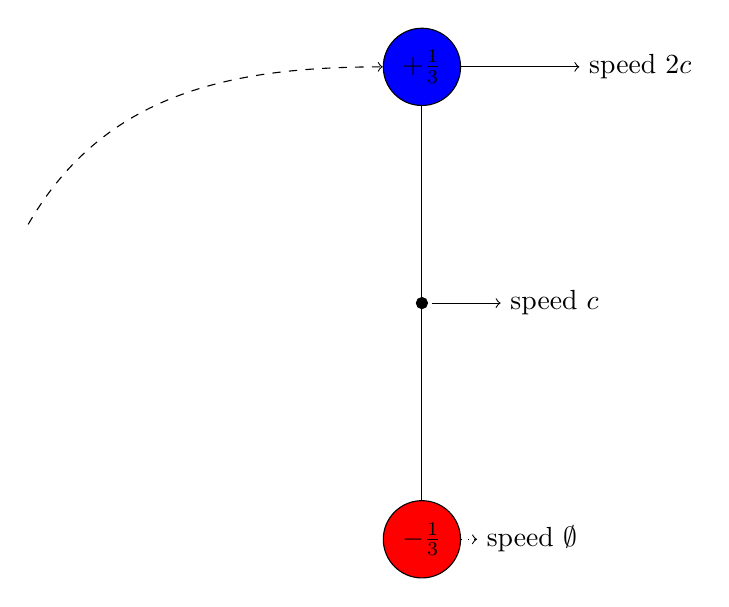
\begin{tikzpicture}[scale=1, rotate=0]

% photon vertical with speed vectors

\path 
(0,0) node[circle,draw, fill=red]  (red) {$-\frac{1}{3}$}
(0,6) node[circle,draw, fill=blue] (blue) {$+\frac{1}{3}$};
\draw[black] (red) -- (blue)         node[pos=0.5](center){};
\filldraw
 (center) circle (2pt);
\draw[->, black] (center) -- ++(1,0) node [anchor=west]{speed $c$};
\draw[->, black] (blue) -- ++(2,0) node [anchor=west]{speed $2c$};
\draw[->, dotted] (red) -- ++(0.7,0) node [anchor=west]{speed $\emptyset$};

\draw[->,dashed] (-5,4) to[out=60,in=180] (blue);

\end{tikzpicture}
\caption{Photon vertical with speed vectors 
\label{fig:photon_vertical}}
\end{figure}
